\documentclass[runningheads]{llncs}
\usepackage[T1]{fontenc}
\usepackage{graphicx}
\usepackage{subcaption}
\usepackage[UTF8]{ctex}
\usepackage{enumitem}


\usepackage{changes}  % 使用changes宏包
% \usepackage[final]{changes} % 禁用修订,输出最终修订完成的版本
% \usepackage[commandnameprefix=always, defaultcolor=red]{changes}  % 使用changes宏包
\definechangesauthor[name={zheliku}, color=blue]{zheliku} % 修订作者

\bibliographystyle{splncs04}

\AtBeginDocument{%
  \providecommand\BibTeX{{%
    Bib\TeX}}}

\begin{document}

\title{VRTI:支持被动触觉的手势交互,增强沉浸式学习体验}

% \author{Hailin Ji\inst{1} \and 
% % \orcidID{0009-0002-3512-6730} 
% Yihang Li\inst{1} \and 
% Yiran Zhang\inst{1} \and 
% Hongwen Zhang\inst{1} \and 
% Xiaoyan Hu\inst{1} \and 
% Yanhong Luo\inst{2}}
 
% \authorrunning{H. Ji et al.}

% \institute{Beijing Normal University, Beijing, China \and
% Northwest Minzu University, Beijing, China}

\author{匿名作者}

\maketitle

  % 实时传感网络通过时空同步将物理道具的静态属性转化为动态反馈。
  % 2) \textbf{手势-道具一致性模型}:实现视觉-触觉同步交互,支持手部操作期间的交互校准。

\begin{abstract}
在沉浸式学习环境中使用手势交互(GI)能够提供直观的学习体验,但缺乏力触觉反馈显著削弱了其沉浸感。传统的主动触觉方案限制GI的交互灵活性,被动触觉方案则难以满足动态交互需求。针对上述问题,本文提出虚拟-现实孪生交互(Virtual-Reality Twin Interaction, VRTI)框架,采用动态被动触觉(DPHF)与触觉重定向(HR)技术,为手势交互提供动态被动触觉反馈。同时,
% 针对VRTI设计基于手势预测与预交互库的手部重定向方案,实现视觉与触觉同步。此外,
基于VRTI开发了支持抓握、按压和捏合三种基本操作的VR孪生体原型系统,并应用于沉浸式学习环境。最后,选取64名高中生进行用户研究,结果表明,与GI组相比,VRTI组显著提升了用户的学习动机(p<0.001)与临场感(p<0.001)。

\keywords{虚拟现实 \and 被动触觉反馈 \and 沉浸式学习 \and 手势交互 \and 手部重定向}
\end{abstract}

\section{引言}
手势交互(GI)作为虚拟现实(VR)中最自然的交互方式之一,在沉浸式学习环境中展现出显著优势\cite{fang2024interactive,amaral2024interactive}。然而,当前以视觉为主导的交互范式存在关键局限——缺乏真实的触觉反馈。这一缺陷严重制约了虚拟现实在教育应用中的沉浸感和交互效果。

目前主流的触觉反馈解决方案可分为两类:主动式和被动式。主动式触觉利用系统控制的执行器主动对用户施加力(如力反馈手套),提供动态范围的触觉反馈,但其设备笨重、交互受限的特点限制了在教育场景中的普及应用\cite{bonfert2023challenges,shigeyama2019transcalibur}。被动式触觉通过在虚拟对象位置处放置实体物理对象(也称为代理或道具),使用户触摸实体表面获得触觉\cite{hinckley1994passive},然而现有被动触觉方法多依赖静态道具\cite{strandholt2020knock,fang2023vr,rettinger2023touching},这些道具无法适应沉浸式学习环境中常见的动态交互需求。

近年来,动态被动触觉(Dynamic Passive Haptic Feedback, DPHF)技术为解决这一困境提供了新的可能性\cite{zenner2017shifty}。其使用执行器来改变被动触觉属性(例如大小、形状、重量、重量分布、纹理、温度、位置、方向、功能等),而不会对用户施加明显的主动力,使其能够适应用户的交互需求,从而提供更自然的触觉反馈。与传统的被动触觉代理相比,DPHF代理会根据其所代表的虚拟物体调整其被动触觉响应,从而提高VR交互的触觉真实感。André Zenner等人首次将DPHF与触觉重定向(HR)结合,发现二者的结合使用能让用户更不易被察觉触觉错位,证明了DPHF技术与HR的结合具有显著的应用潜力\cite{zenner2021combining},但相关研究目前仍处于起步阶段。

综上所述,本研究的主要贡献如下:

\begin{enumerate}[label={\arabic*)}]
  \item 提出虚拟-现实孪生交互(VRTI),一个融合手势交互的DPHF/HR方案,支持灵活的手势交互操作与动态触觉反馈。
  \item 设计基于VRTI的DPHF与HR方案,实现视觉与触觉同步。
  \item 基于VRTI实现三种VR孪生体(拉杆、按钮和旋钮),分别支持抓握、按压和捏合操作,并应用于高中动量守恒定律的沉浸式学习环境。
  \item 通过用户研究(N=64)证明VRTI的有效性:与传统手势交互(GI)相比,VRTI显著提升了用户的学习动机(p<0.001)与沉浸感(p<0.001)。
\end{enumerate}

\section{相关工作}
\subsection{手势交互} 
手势交互作为人机交互领域的重要研究方向,通过识别上肢姿势或运动实现意图表达与操作控制\cite{yang2019gesture},在虚拟现实(VR)和增强现实(AR)等沉浸式环境中展现出显著优势\cite{10574578}。相关研究表明,与身体其他部位相比,手在传递信息和执行任务中的灵巧性和可操作性使其成为人机交互的理想工具\cite{karam2006framework}。其核心价值体现在三个方面\cite{mitra2007gesture,10580881,app14114935}:一是灵巧性,用户无需额外硬件即可通过手部动作完成交互,降低了操作摩擦;二是即时性,能与VR设备深度集成实现无缝识别;三是自然与直观性,通过模拟真实手部动作(如抓取、旋转)增强交互体验。

手势设计需遵循用户导向、文化适配、系统一致性和实时反馈等原则\cite{lou2018analysis}。例如,Wu Y等人提出的11种基础手势集(如捏合、抓握、旋转)明确了常见操作任务的映射关系\cite{wu2024empirical},而Herbert O M则通过静态/动态分类区分信息传递与复杂动作控制\cite{herbert2024static}。在虚拟现实领域,手势交互已广泛应用于沉浸式游戏控制和教育培训等场景\cite{10574578,lu2024chemical},显著提升用户沉浸感和交互效率\cite{10580881},且有助于增强学习动机和知识掌握\cite{lu2024chemical}。

然而,手势交互仍存在以下限制\cite{herbert2024static,app14114935}:一是传感器局限,遮挡和光照变化会导致跟踪失效;二是意图歧义,因自然对话中手势的随意性难以精准解析用户目标;最后是缺乏触觉反馈,导致用户感官刺激不足,降低操作虚拟对象时的沉浸感。

\subsection{被动触觉}
虚拟现实中的触觉技术可分为两大类:主动触觉和被动触觉。主动触觉技术使用机械和电子控制装置,通过马达、液压或气动系统生成可控的物理力,作用于用户的手部或身体,从而模拟真实环境中的力触觉反馈\cite{vaghela2021active}。被动触觉是一种将物理道具或环境重新用于在VR和AR中创造触觉感的技术,最早由Insko等人提出\cite{insko2001passive}。它利用物理代理通过形状向用户传递反馈,从而为虚拟物体赋予实体维度。被动触觉技术使用户能够更灵活、更精确地控制和操作3D虚拟模型,无需特殊触觉设备,因此具有高度适应性和可部署性\cite{henderson2008opportunistic,shapira2016tactilevr,10.1145/3313831.3376313}。

被动触觉反馈的实现主要面临以下2个挑战。首先,如何设计和制造适物理代理,使其在触觉特性上足够相似。其次,如何在虚拟环境中实现与物理代理的精确对齐,以实现无缝交互\cite{zenner2021combining}。此外,被动触觉技术通常需要用户与物理代理进行直接接触,这可能会限制其在某些应用场景中的使用。近年来,动态被动触觉(DPHF)技术成为被动触觉领域的重要发展方向。这类技术通常结合实时传感与执行器(如电机、致动器),在用户交互过程中自动调整物理代理状态,实现虚拟与现实的高保真同步。DPHF通过集成可变形、可移动或可调节的物理代理,使其触觉属性(如位置、形状、阻力等)能够根据虚拟环境需求动态变化,增强用户的沉浸感和交互兴趣\cite{zenner2017shifty}。

% DPHF显著提升了被动触觉的灵活性和适应性,支持复杂动态交互场景(如多步骤实验、连续操作任务),并能与视觉、听觉等多模态反馈协同增强沉浸体验。

\subsection{沉浸式学习}
随着虚拟现实技术的发展,其在沉浸式学习中的应用日益广泛,大多数研究涵盖 STEM(科学、技术、工程、数学)主题\cite{georgiou2021learning,campos2022impact,prahani2022trend,informatics9040075,virtualworlds3040026}。沉浸式学习环境能够让学生以第一视角参与学习体验,促进学生理解实验现象,提升学习的效率和动机\cite{varela2017embodied}。然而,大多数研究和实践聚焦于使用视觉反馈传递信息,而忽视其他感官的交互。

近年来,带有力触觉的沉浸式学习环境逐步受到关注\cite{10.1145/3593429,shen2023research,johnson2023embodied},这些环境能够提供关于物体形状、纹理、温度和重量等信息,增强学习体验的真实感和沉浸感\cite{varela2017embodied}。目前,支持触觉反馈的沉浸式学习环境主要分为3类:基于力触觉反馈设备的主动触觉\cite{qi2020impact,acevedo2022effects}、基于物理道具的被动触觉\cite{10.1145/3593429}和基于标记的增强现实\cite{knierim2020tangibility,liu2021effects}。其中,用于主动触觉的常见力触觉反馈设备包括触觉反馈操纵杆/机械臂(如PHANTOM系列)、触觉手套(如HaptX手套)和振动设备(如VR控制器)。被动触觉常使用物理道具(如球体、立方体等)提供触觉反馈,用户通过触摸这些道具感知虚拟物体的属性。增强现实技术则通过在用户视野中叠加虚拟标记或图像,提供额外的触觉信息。触觉反馈在沉浸式学习中的应用已被多项研究证实,能够显著提升学生对虚拟实验的兴趣和参与度\cite{qi2020impact},并有效提高学生的实验操作准确性和效率\cite{acevedo2022effects}。

尽管沉浸式学习环境能够改善学习者的学习体验,其设计仍需理论指导以辅助提升教学效果\cite{matovu2023immersive,marougkas2023virtual}。常见学习理论包括认知负荷理论\cite{sweller1988cognitive}、ARCS动机模型\cite{keller1987development}和沉浸理论\cite{sherman2003understanding}。其中,认知负荷理论(Cognitive Load Theory, CLT)强调学习过程中认知资源的有效管理,ARCS动机模型(Attention, Relevance, Confidence, Satisfaction)则关注学习动机的激发与维持,而沉浸理论则探讨用户在虚拟环境中的沉浸感和参与度。通过将这些理论应用于沉浸式学习环境设计,教育者可以更好地理解学习者的认知负荷、动机和沉浸感,从而优化教学策略和内容。

\section{VRTI}
我们提出VRTI交互框架,其核心是VR孪生体(Virtual-Reality Twin, VRT),由一对物理世界中的真实交互对象(Real Interaction Object, RIO)与其在虚拟环境中的对应虚拟交互对象(Virtual Interaction Object, VIO)组成。RIO采用DPHF技术,集成传感器与执行器,为用户提供动态被动触觉反馈;VIO在虚拟场景中与RIO实时同步,并融合手势追踪与HR技术,支持多种手势交互,提供与触觉同步的视觉反馈。

\subsection{概念验证}
针对抓握、按压和捏合3种手势,我们设计了以下3种VRT进行验证:

\begin{enumerate}[label={\arabic*)}]
  \item \texttt{拉力器} 提供抓握手势交互,反馈与拉动距离成正比的张力;
  \item \texttt{按钮} 提供按压手势交互,反馈与按压距离成正比的弹力;
  \item \texttt{旋钮} 提供捏合手势交互,反馈捏合轻小物体的触觉。
\end{enumerate}

图\ref{fig:interaction-flow}展示三者的交互流程。在抓握交互中,用户握住滑块,向后拉动弹簧至特定距离触发拉杆,释放滑块使弹簧回弹完成交互;在按压交互中,用户将手置于开关上方,按压至特定距离激活按钮,抬手完成交互;在捏合交互中,用户手指捏住手柄头部,绕中心轴旋转调整角度,松手完成交互。

\begin{figure*}[t]
  \centering
  \includegraphics[width=1\textwidth]{image/Interaction-Flow.pdf}
  \caption{三种VRT交互流程}
  \label{fig:interaction-flow}
\end{figure*}

\subsection{DPHF实现}
VRT的VIO与RIO的数据通信通过实时传感技术实现,借助传感器采集RIO物理属性,经滤波后通过Arduino传输至VIO实现实时更新。图\ref{fig:structural-diagram}展示各部件结构设计。三者RIO与VIO均源自同一3D模型:RIO通过3D打印获得,VIO通过模型导入Unity创建。因用户视觉反馈直接由VIO提供,VIO在虚拟环境中着色渲染,RIO则保持未着色状态。

\begin{figure*}[t]
  \centering
  \includegraphics[width=1\textwidth]{image/Structural-Diagram.pdf}
  \caption{三种VRT结构图}
  \label{fig:structural-diagram}
\end{figure*}

\subsubsection{传感与执行器}
三种VRT配备的传感与执行器介绍如下:
\begin{enumerate}[label={\arabic*)}]
  \item \texttt{拉力器} 针对抓握手势,采用拉力传感器与弹簧的组合。拉力传感器安装于弹簧与物块的连接处,实时检测用户施加的拉力。其采集频率为50Hz,拉力测量范围为0N至20N,精度为±0.1N。弹簧作为简易执行器,在每次拉动后将物体恢复原位。
  \item \texttt{按钮} 针对按压手势,采用薄膜压力传感器与弹簧的组合。薄膜压力传感器放置于弹簧底部,当用户按下按钮时,通过弹簧弹力采集用户压力大小。其传感器的采集频率是100Hz,采集的压力范围是0N~10N,分辨率为0.01N。弹簧同样作为简易执行器,在每次按压后将物体恢复原位。
  \item \texttt{旋钮} 针对捏合手势,采用角度传感器,用于实时检测旋钮的旋转角度。角度传感器安装于旋转轴的中心位置,以50Hz的采集频率捕捉旋钮的旋转状态,角度测量精度为±0.5度。
\end{enumerate}

\subsubsection{数据通信}
鲁棒的通信架构确保RIO的低延迟数据传输。使用Arduino UNO作为接口采集原始传感器数据,经过输入降噪、归一化和状态预测流程,识别数据信号。
\begin{enumerate}[label={\arabic*)}]
  \item \texttt{输入降噪} 卡尔曼滤波应用于原始数据$x$,通过最优结合预测和含噪测量估计真实系统状态。
  \item \texttt{归一化} 将原始数据$x$归一化至统一范围[0,1]得到$\bar{x}=\displaystyle\frac{x-x_{\min}}{x_{\max}-x_{\min}}$。下限$x_{\min}$通常对应RIO初始/静止状态,上限$x_{\max}$通过重复用户试验捕获预期最大值。
  \item \texttt{平滑处理} 使用经验阈值$\varepsilon$检测状态变化,当$\bar{x}>\varepsilon$时表示数据开始输入,$\Delta\bar{x}>\varepsilon$表示状态切换。
\end{enumerate}

\subsection{HR实现}
通过将VIO与RIO进行空间对应,确保虚拟与现实的触觉反馈同步。核心是手部重定向,通过手势识别与预定义交互库实现视觉与触觉的无缝衔接。

\subsubsection{空间校准}
确保VIO与RIO的空间对应对提供真实同步的视觉与触觉反馈至关重要,能够最大化用户体验的沉浸感。RIO以固定空间关系安装在平板上,建立物理参考系。VIO通过定义虚拟单位(Unity单位)与现实单位(米)的比例尺构建,匹配RIO在物理参考系中的相对位置和方向。

\subsubsection{手部重定向}
手势追踪技术会带来估计误差,导致虚拟手与VIO产生视觉穿透。我们为每类VIO预定义交互的标准手势,组成预定义交互库,并定义用户虚拟手为中心的球形边界体积为交互触发区。当VIO进入触发区时,检测当前用户手势。若与预定义交互库中的某个手势匹配,则将虚拟手平滑插值至预设标准姿势以最小化视觉穿透。


\subsection{实验场景}
VRTI框架具备高度灵活性和可扩展性,适用于多种需要同步触觉的沉浸式学习和交互场景,包括但不限于:

\begin{enumerate}[label={\arabic*)}]
  \item \texttt{科学实验教学} 如物理、化学、生物等实验课程,支持力学实验、分子结构操作、微观现象模拟等,提升学生对抽象概念的感知和理解。
  \item \texttt{工程与技能训练} 如机械装配、电子电路搭建、手工艺技能训练等,帮助学习者通过真实触觉反馈掌握操作技巧。
  \item \texttt{医学仿真与康复训练} 如外科手术模拟、康复动作训练等,增强医学生和患者的操作体验与学习效果。
\end{enumerate}

本研究针对沉浸式学习场景,将3种VRT应用于设计动量守恒定律探究实验。该定律涉及力学基本原理,具有较强的实验操作性和抽象性。同时,实验需要学生通过实际操作滑块、弹簧等物理器材,体验力与运动的关系,包含抓握、按压和捏合的典型手势操作。

具体实验场景如图\ref{fig:experiment-scenario}所示。物块A(红色)和物块B(黄色)通过一根弹簧相连,构成弹簧双振子系统,置于无摩擦、无外力的光滑平面上。左侧为图像切换面板,包含速度-时间($v-t$)图像、动量-时间($P-t$)图像、能量-时间($E-t$)图像三个按钮,用于切换显示的时序物理量图像。右侧为物理参数面板,用于自由调节两物块的质量($m_A$和$m_B$)、弹簧劲度系数($k$)。后侧为数据显示面板,左半部分显示系统速度、动量和能量的实时图像,右半部分则显示其对应推导公式,帮助学生理解记忆。左下角则提供三种图像切换的交互方式。

\begin{figure*}[t]
  \centering
  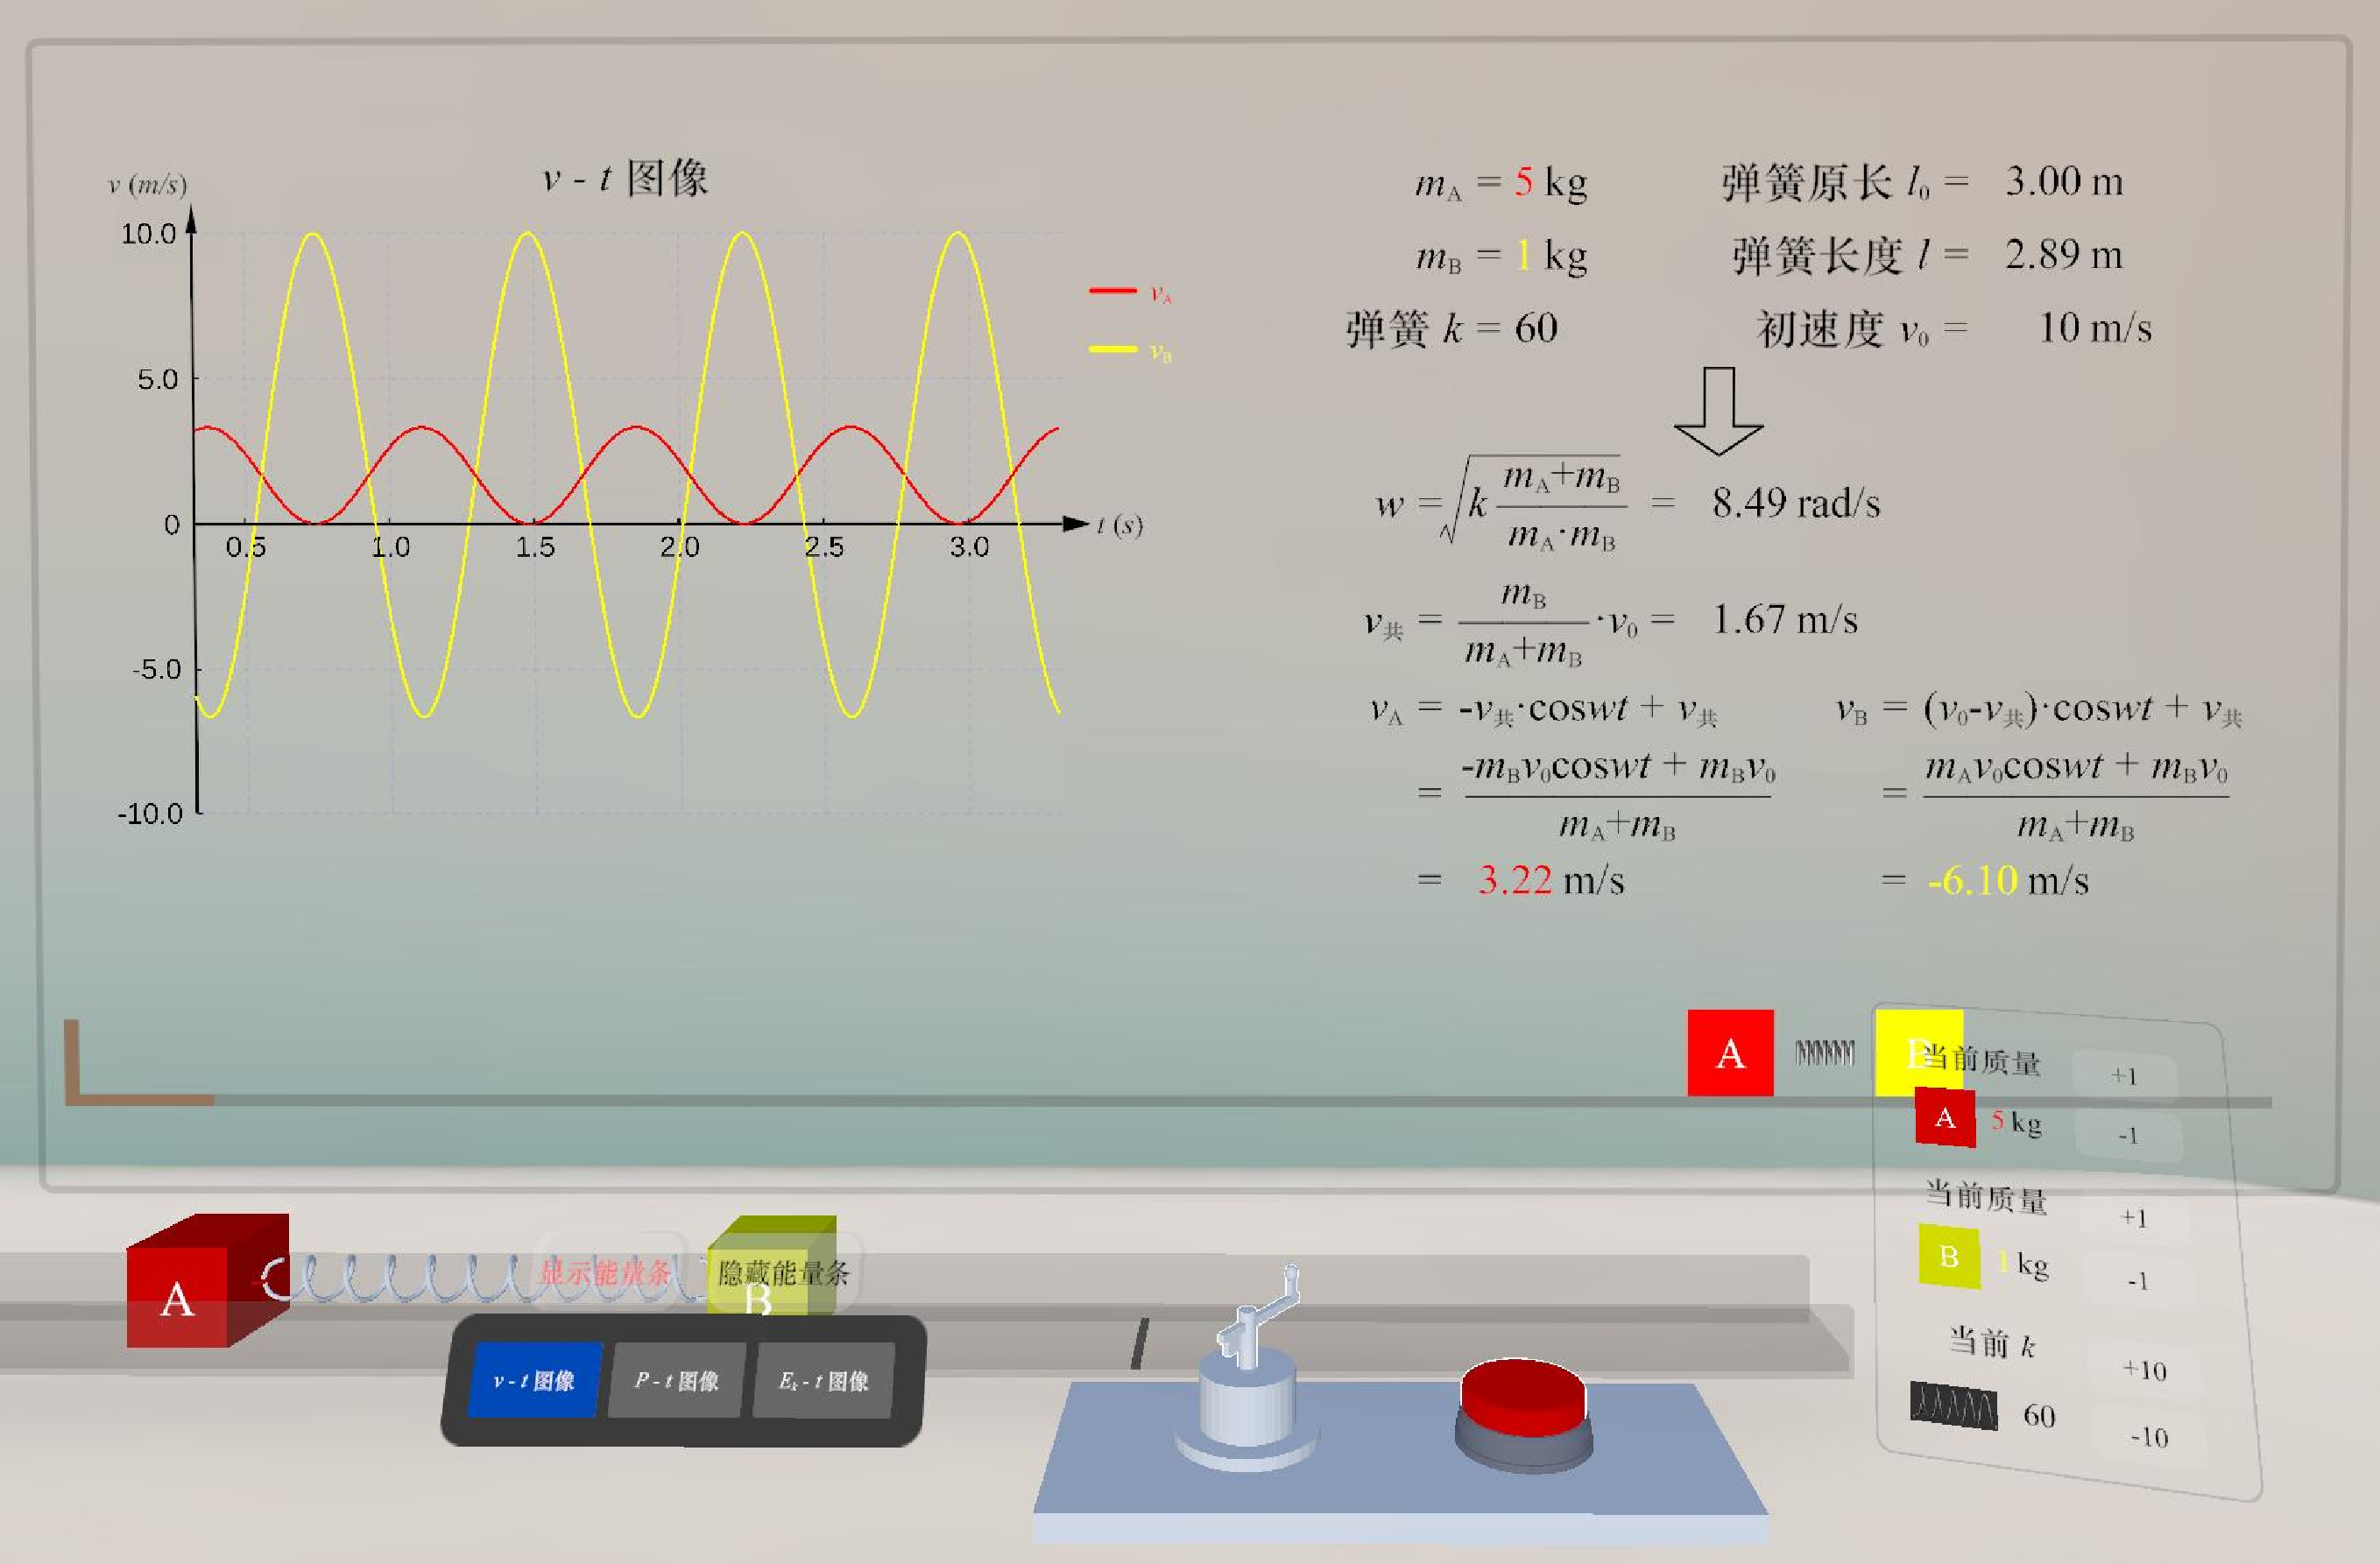
\includegraphics[width=1\textwidth]{image/experiment-scenario.pdf}
  \caption{实验场景}
  \label{fig:experiment-scenario}
\end{figure*}

% 进入实验场景后,学生首先用食指点击右侧参数设置面板按钮配置实验参数(含两滑块质量和弹簧劲度系数)。随后将B滑块向右拉动至适当力度释放,"发射"B滑块并观察系统运动。接着旋转旋钮调整运动过程时间线(顺时针前进/逆时针后退),探索可视化面板图像特征和物理量关系。最后当系统到达终点位置时按下按钮重置系统并重新配置参数继续探索。

\section{评估}
\subsection{假设}
比较VRTI和GI两种交互方式。基于先前相关触觉研究,我们作出以下假设:

\begin{itemize}[label=$\bullet$]
  \item {\textbf{H1}}:在手势交互中增加触觉反馈能使手势交互增强学生对实验的兴趣和参与度,提升学习动机。即,VRTI在学习动机方面显著高于GI。
  \item {\textbf{H2}}:在手势交互中增加触觉反馈能增强学生的沉浸感,使其更深入地参与实验过程。即,VRTI在沉浸感方面显著高于GI。
\end{itemize}

\subsection{方法}
针对假设\textbf{H1},采用Keller量表\cite{keller1983motivational},基于ARCS动机模型评估四个维度:注意力、相关性、信心和满意度,衡量学习者参与和完成学习任务的内驱力。

% 接触触觉反馈等新技术时,学习者的内在动机(如好奇心和探索欲)或外在动机(如任务完成奖励)可能显著影响其参与度和学习效果。更高动机增加学生克服挑战的可能性,从而有效利用触觉反馈技术学习。

针对假设\textbf{H2},采用Schubert量表 \cite{schubert2001experience},聚焦虚拟环境中的临场感,通过空间临场感、参与度和虚拟环境真实感三个维度综合评估学生沉浸感和控制感。

所有量表均经翻译和本地化确保适合本实验文化和教育背景。此外,在参与者结束实验后,我们随机抽取部分参与者进行半结构化访谈,以收集对VRTI的主观体验和反馈。

\subsection{实验}
实验使用Meta Quest 3作为VR头显提供视觉信息,VR孪生体作为交互方式提供触觉反馈。程序交互逻辑和可视化场景通过Unity 2021.3.32f1c1实现。VR孪生体采用手势追踪技术将用户物理手可视化为虚拟手进行交互,通过传感技术实现实时数据更新与同步。手势追踪通过Meta XR All-in-One SDK (v63)实现。实验交互框架如图\ref{fig:system-framework-flowchart}所示。

\begin{figure*}[t]
  \centering
  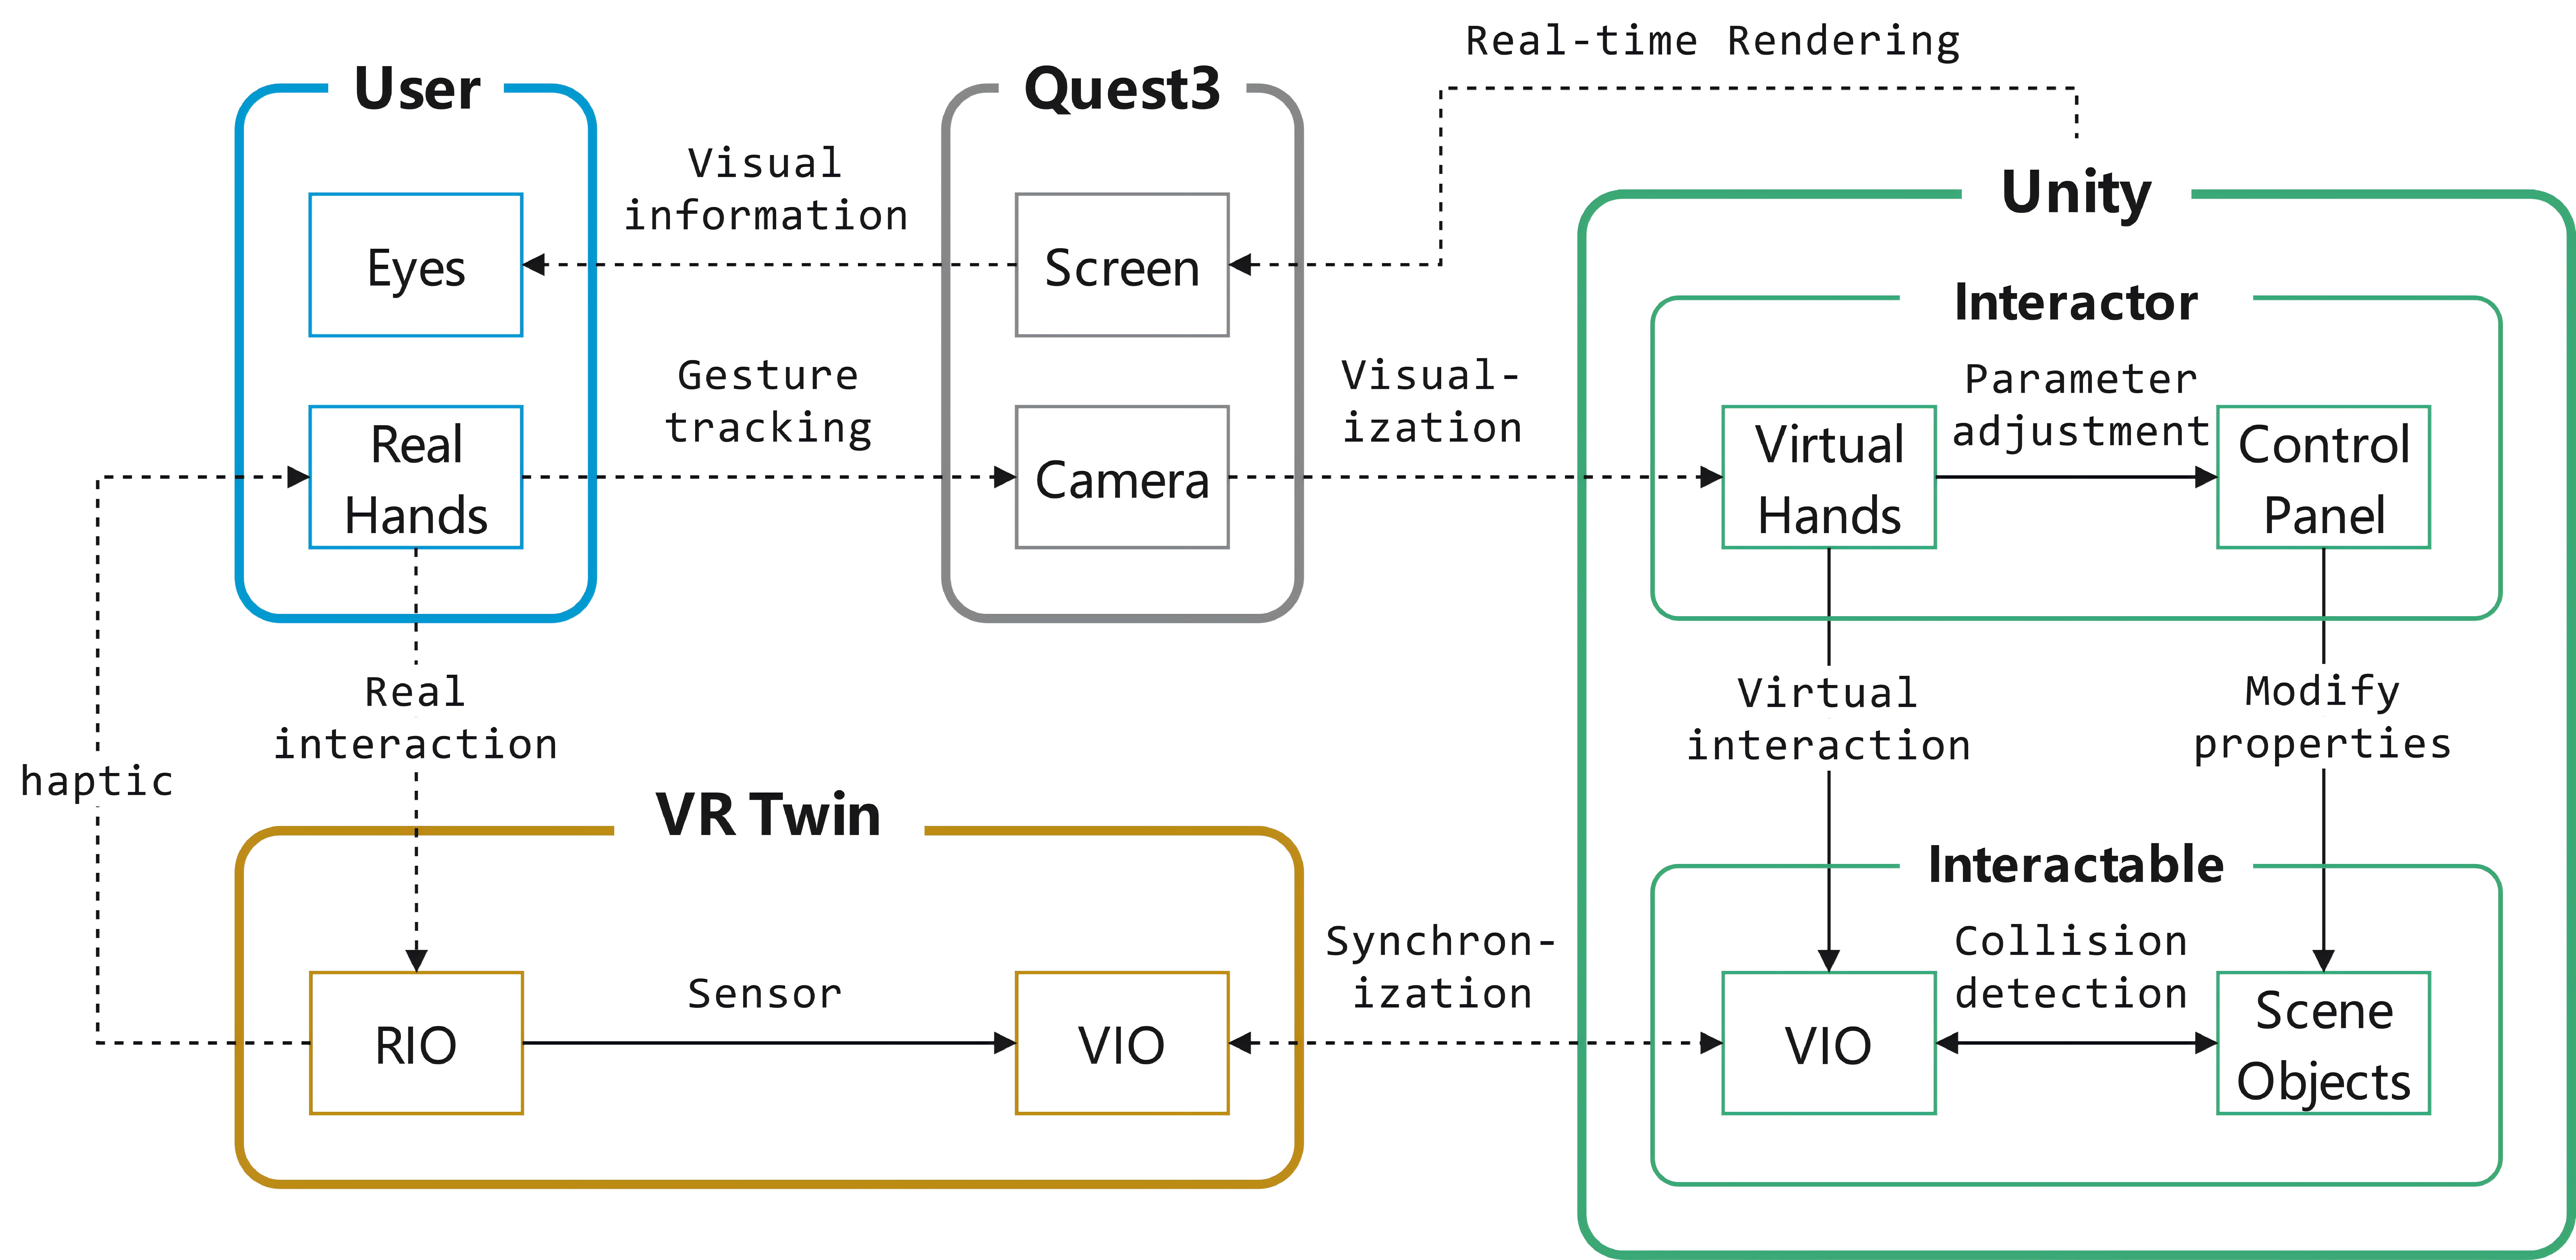
\includegraphics[width=1\textwidth]{image/system-framework-flowchart.pdf}
  \caption{实验交互框架}
  \label{fig:system-framework-flowchart}
\end{figure*}

\subsection{流程}
\subsubsection{参与者}
当地招募XXX学校64名高中生参与实验。参与者年龄范围在16岁到18岁之间。所有参与者的视力正常或矫正为正常。参与者被随机均分两组,实验组(N=32)使用VRTI交互,对照组(N=32)使用传统手势交互(GI)。

\subsubsection{实验步骤}
学生进入实验后:

\begin{enumerate}[label=$\bullet$]
  \item 首先,通过右侧物理参数面板调整物块A、B的质量和弹簧劲度系数。
  \item 其次,做出抓握手势抓住右侧物块B,向右方拉动一定距离并释放,使物块B在弹簧拉动下获得初速度,系统随之进行周期性运动,A、B物块上方分别显示瞬时速度矢量与合外力矢量。
  \item 再次,做出捏合手势握住手柄旋转旋钮,控制时间的推进或倒退,使弹簧双振子系统静止在某一时间点。顺时针旋转旋钮推进系统时间;逆时针旋转旋钮则使系统时间倒退。
  \item 最后,做出按压手势按下按钮,系统将从当前时间点开始继续运行。当系统处于运动状态时,按下按钮则会使系统恢复到初始状态。
\end{enumerate}

\subsubsection{监督与指导}
为确保结果有效性,所有参与者实验前接受统一实验介绍和操作指导,并配备助教监督以确保每位参与者遵循实验步骤,如图\ref{fig:experimental-procedure}所示。流程含以下四步:

\begin{enumerate}[label={\arabic*)}]
\item \texttt{实验介绍} 学生观看指导视频熟悉实验操作流程。
\item \texttt{实验操作} 学生按分组进行实验。
\item \texttt{后测} 学生独立完成用户体验问卷,包含10项学习动机和12项沉浸感调查。
\end{enumerate}

\begin{figure}
  \begin{subfigure}{0.48\linewidth}
    \centering
    \includegraphics[width=\linewidth]{image/experimental-introduction.pdf}
    \caption{}
    \label{fig:experimental-introduction}
  \end{subfigure}
  \hfill
  \begin{subfigure}{0.48\linewidth}
    \centering
    \includegraphics[width=\linewidth]{image/experimental-operation.pdf}
    \caption{}
    \label{fig:experimental-operation}
  \end{subfigure}
  \caption{实验演示。(\subref{fig:experimental-introduction})实验介绍,(\subref{fig:experimental-operation})实验操作}
  \label{fig:experimental-procedure}
\end{figure}

\subsection{结果分析}

为验证假设$\textbf{H1}$和$\textbf{H2}$,我们使用Shapiro-Wilks检验实验组和对照组数据,结果显示均不服从正态分布,故采用Mann-Whitney U检验分析组间差异。以下数据中,显著性水平$p \le 0.05$ (*)表示显著差异,$p \le 0.01$ (**)表示高度显著差异,$p \le 0.001$ (***)表示极其显著差异。效应量解释:$|r| \le 0.1$为小效应,$0.1 < |r| \le  0.3$为中效应,$d > 0.5$为大效应。

图\ref{fig:user-experience-result}对比两组在学习动机和沉浸感方面的实验结果。各组上方实心圆点为样本点,核平滑拟合曲线描述其分布。下方I型箱线图展示25\%(Q1)、50\%(Q2)和75\%(Q3)分位数。实验组的学习动机($Z=-3.509,p<0.001,|r|=0.620$)与沉浸感($Z=-4.751,p<0.001,|r|=0.840$)具有显著提升,为大效应。因此我们有充分的理由接受假设$\textbf{H1}$和$\textbf{H2}$。在实验过程中,所有参与者均没有报告任何不适或晕动症状,且没有感知到手部重定向的存在。

\begin{figure*}[t]
  \centering
  \includegraphics[width=0.75\textwidth]{image/user-experience-result.pdf}
  \caption{VRTI组与GI组在学习动机和沉浸感方面的结果对比}
  \label{fig:user-experience-result}
\end{figure*}

进一步分析学习动机和沉浸感,发现VRTI组在学习动机的4个维度与沉浸感的3个维度均显著优于GI组,结果如图\ref{fig:three-user-experience-result}所示。

\begin{figure*}[t]
  \centering
  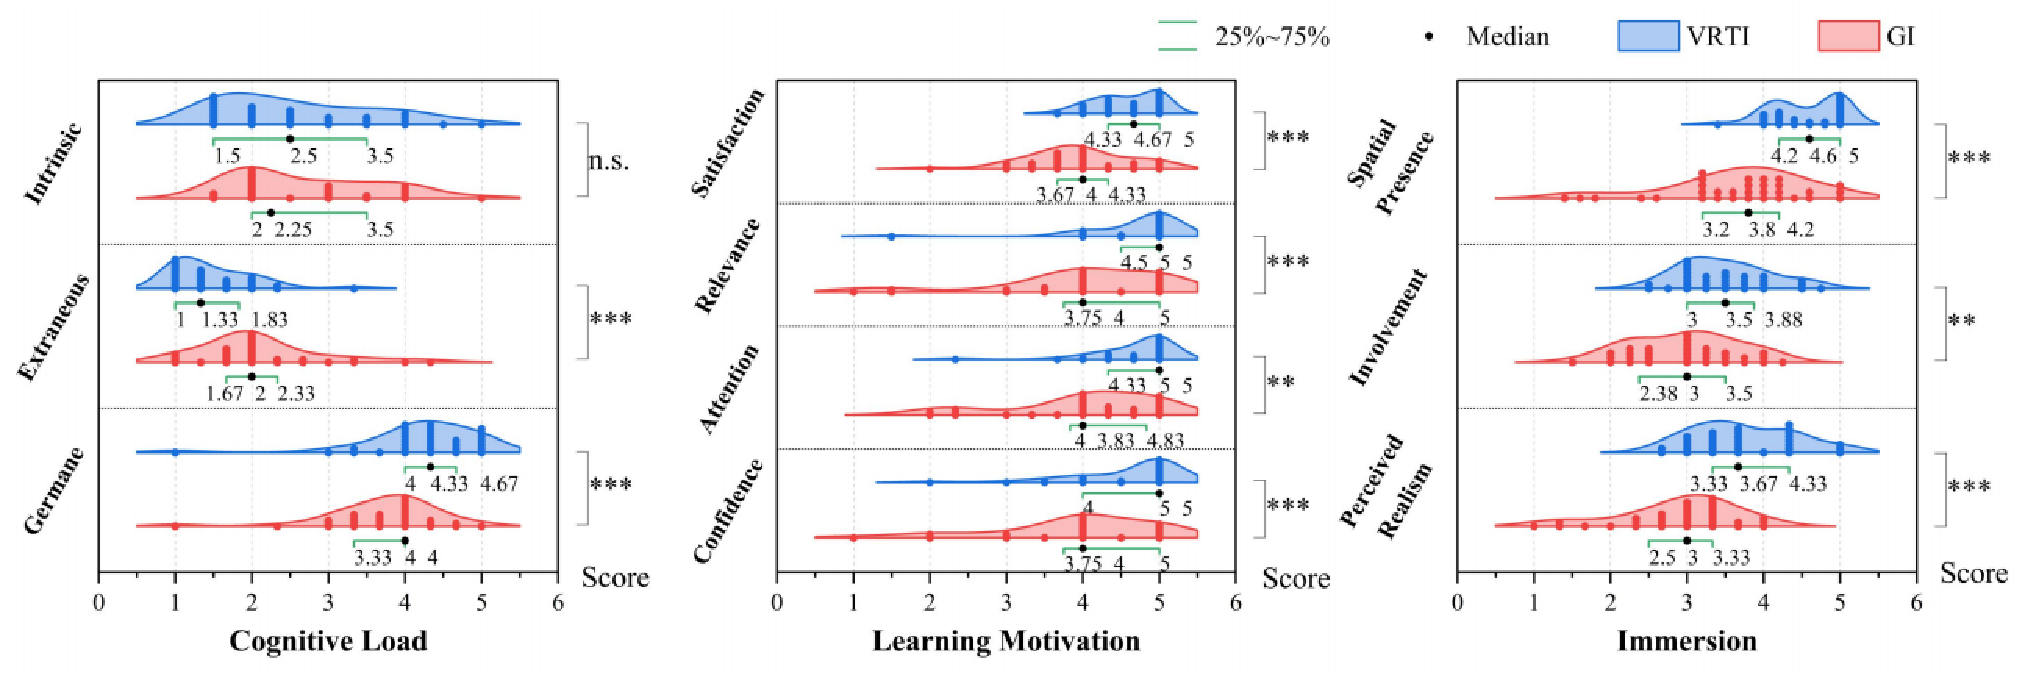
\includegraphics[width=\textwidth]{image/three-user-experience-result.pdf}
  \caption{VRTI与GI各用户体验维度对比}
  \label{fig:three-user-experience-result}
\end{figure*}

\subsubsection{学习动机}
在注意力维度($Z=-3.382, p=0.001, |r|=0.598$)上,VRTI的触觉反馈能更好吸引学生注意力,减少分心;在相关性维度上($Z=-3.313, p=0.001, |r|=0.586$),VRTI组的学生更易将虚拟实验与现实知识联系起来,增强学习内容的实际意义;在信心维度($Z=-3.001, p=0.003, |r|=0.531$)上,VRTI的触觉反馈帮助学生更自信地完成实验任务,降低操作难度;在满意度维度($Z=-4.127, p<0.001, |r|=0.730$)上,VRTI组的学生对整体学习体验更加认可和满意。

\subsubsection{沉浸感}
在空间临场感维度($Z=-4.021, p<0.001, |r|=0.712$)上,VRTI的同步触觉反馈使学生更容易感知自身与虚拟环境的空间关系,增强“身临其境”的体验;在参与度维度($Z=-3.765, p<0.001, |r|=0.667$),VRTI组学生在实验过程中表现出更高的主动参与和持续投入,交互过程更具吸引力;在虚拟环境真实感维度($Z=-4.512, p<0.001, |r|=0.800$),VRTI的动态触觉反馈显著提升了虚拟实验的真实感和可信度。

\subsubsection{半结构化访谈}
结合用户访谈,部分学生反馈VRTI系统的真实触觉体验让他们“仿佛在做真实实验”,更愿意沉浸其中并专注于实验任务,主动探索和反复操作。与传统GI组相比,VRTI组学生在实验过程中表现出更强的主动性和探索欲望,愿意尝试不同参数设置和交互方式,整体沉浸体验更佳。这些结果进一步验证了VRTI在提升学习动机和沉浸感的有效性和应用潜力。

\section{讨论}
\subsubsection{推进自动校准}
当前VR孪生系统中RIO和VIO的部署仍属半自动化,需手动调整确保精确对齐。本研究期间VR头显功能限制导致难以捕捉摄像头图像实现自动定位。仅依赖传感技术精确定位成本高昂且可能引入额外基站部署,增加系统复杂性。未来研究将探索全自动部署方法,使用户佩戴VR头显后即刻实现RIO精确定位和VIO实时重建。通过集成先进计算机视觉技术和机器学习算法,实现对齐误差的动态预测与调整,达成无需人工干预的空间对齐。

\subsubsection{道具耐久性}
用户反馈还凸显触觉反馈设备耐久性和长时间交互的身体疲劳问题,可能影响系统长期可用性和用户满意度。未来研究将优先提升交互设备耐久性,采用先进材料改善触觉反馈设备寿命和响应性,同时融入人机工学设计原则减少用户交互负担。

\subsubsection{道具耐久性}
最后,当前系统的实验设置和用户交互依赖预定义规则,限制了其对多样化学习场景和个性化学习需求的适应性。未来研究将聚焦AI与VRTI的集成,分析用户行为、预测学习需求并动态调整实验环境。例如AI可引导用户完成复杂实验,提供个性化反馈并根据进度推荐补充学习资源。AI驱动的数据分析还可评估学习效果,为系统和课程改进提供依据。

\section{结论与未来工作}
本文针对VR沉浸式学习环境中手势交互(GI)缺乏触觉反馈的问题,提出虚拟-现实孪生交互(VRTI)。针对高中物理学习中的动量守恒实验,设计实现支持抓握、按压和捏取操作的三种虚拟-现实孪生体(VR孪生体)。在动量守恒实验场景中对比评估VRTI与GI表明,前者显著提升用户学习动机和沉浸感且未显著增加认知负荷,同时更好帮助用户理解实验内容并提升知识综合应用能力。未来研究将探索VR孪生体在其他物理学习场景的应用,改进硬件结构并优化交互方式以提升用户学习体验和操作舒适度。

\begin{credits}
\subsubsection{\ackname} 
\deleted{本研究得到国家自然科学基金(编号62377004)支持。}

\subsubsection{\discintname}
作者声明无利益冲突。
\end{credits}

% \setlistofchangestitle{修订历史}
% \listofchanges

\bibliography{VRTI-bib}

\end{document}